\chapter{Application Logic}

\section{General Technologies and Frameworks}

As it is a web application, HTML, CSS and JavaScript were used for the client side of the application, although this was augmented with both JQuery and Bootstrap to ease the development of the Javascript and the CSS respectively. 

For the server side of the application, the code was written in python, using the Flask framework and its integrated technologies. Flask was used as it is easier to user then the alternative python frameworks and the developer has experience using it. python was also chosen for similar reasons and due to the fact that the developer likes it. The memory usage and speed of the various possible programming languages and frameworks was not considered. Ease of use and familiarity were the primary considerations. 

\section{Article Discovery}

For the article discovery portion of the application, the need was for a list of articles, from a variety of sources about a variety of topics. The solution that was found after some search on the internet, was Google News.

Google News provides several lists of recent articles from different sources divided in different topics, additionally, each of these lists is provided in an RSS feed XML file, a format that allows the code to be written for both URL and title extraction with minimal effort, both on the parts of the developer and the machine life time.

The categories provided by the Google News RSS feeds were usable, but overall they were fairly common news categories. On the plus side, these categories are recognisable, on the down side, these categories are not customisable, however, the categories were pre-selected, saving time on artificial category creation, the end user can just selected one of them. 

There were alternatives to the Google News RSS feeds that were examined, primarily \textcite{newsapi}. However this was found to be lacking for two reasons. Primarily, this API would list content, where the primary means of communication was not text. Comics and other image based got added to the lists being provided by the API. As the parser and the gloss system relied on the content being text based and there was no easy way to distinguish being text based content and image based content. The other more minor reason that \textcite{newsapi} was disregarded was because it was more difficult to categorise the articles, whereas the Google News RSS feeds provided pre-created categories, to save time on both filtering out image-based content and the categorisation of articles, the decision was made to use the Google News RSS feeds. 

The end result of this is an application is that the articles being listed in the article selection view are pulled from the Google News RSS feed that corresponds to the category selected by the end user.

\section{Article Difficulty Rating}

The difficulty rating of the article is calculated using two things, the article text as well as the user's experience level. The user's experience level is obtained from the form the user submitted at the start, while the article text needs to be extracted from the article web page and then analysed.

To extract and then analyse the article, two technologies are used. The first is an article scraping python library called \textcite{newspaper}, the purpose of it is to extract the raw article text from the article web page, making the analysis of it easier. Analysis of the article text is then done through another python library called SpaCy, SpaCy is a parts-of-speech tagging library, with some additional advanced features, pretty much all the analysis is performed when the article text is parsed into the library, meaning that library provides a bunch of information about the text.


\section{Gloss Creation}

For the gloss to work, each word of the text is wrapped in a set of span tags. Javascript is then added to the page, which adds an "on click" method to each of the words. When the user then clicks on the word, a request is sent to the application, for a gloss of that particular word in that particular part of speech, where the part of speech is stored in the data labels of the span tags, so this is also submitted to the application.

The application then looks up the translation as well as more in depth grammatical information, once it has this information, it will format it into a pre-prepared html template which is then inserted into the html of the page.

\subsection{Translation Lookup}

For the translation section of the gloss creation, various possibilities were considered, These included online translation services such as \textcite{googletranslate} and \textcite{bingtranslate}, raw datasets such as the \textcite{dictCC} and Dictionary APIs such as the \textcite{oxford} and the \textcite{collins}. 

The technology that would be used in the project would have to:
\begin{itemize}
\item Be able to translate single words from to English
\item Provide Lexical information of those words
\item Be allowed for the content to be hosted and provided through a web interface
\item Be available for less than \pounds150 total
\end{itemize}

The five technologies cited above were checked against these criteria and the results are show in Table \ref{tbl:comp}

\begin{table}
\centering
\caption[Comparison of Translation Software]{Comparison of various translation solutions to see whether or not they fulfil the criteria of the application. }
\label{tbl:comp}
\begin{tabu} to \textwidth{|X[c]|X[c]|X[c]|X[c]|X[c]|}
\hline
\textbf{Product}        & \textbf{German to English Translations} & \textbf{Lexical Information} & \textbf{Allowed Online} & \textbf{Less Than \pounds150  (total)} \\ \hline
Google Cloud Translate  & Yes                                     & No                           & Yes                     & No                               \\ \hline
Microsoft Translator    & Yes                                     & No                           & Yes                     & No                               \\ \hline
Dict.cc Dataset         & Yes                                     & Yes                          & No                      & Yes                              \\ \hline
Oxford Dictionaries API & Yes                                     & Yes                          & Yes                     & Yes                              \\ \hline
Collins Dictionary API  & Yes                                     & Yes                          & Yes                     & No                               \\ \hline
\end{tabu}
\end{table}

As \textcite{oxford} was the only technology to clear all four criteria, the decision was made to used it for development of the application, however other technologies were used in testing the resulting code.

\textcite{oxford} is a REST API where two calls are required to get the desired information. The first, gets the translations of the root words, at the same time this is used to check if a word is the dictionary, the second call, which is made if a translation is found is to get the reasons why that particular mutation from the root occurred.  The process is illustrated in the systems flow diagram in figure \ref{fig:odsf}

\begin{figure}
	\caption{Systems Flow Diagram of the Oxford Dictionaries API}
	\label{fig:odsf}
	\begin{center}
	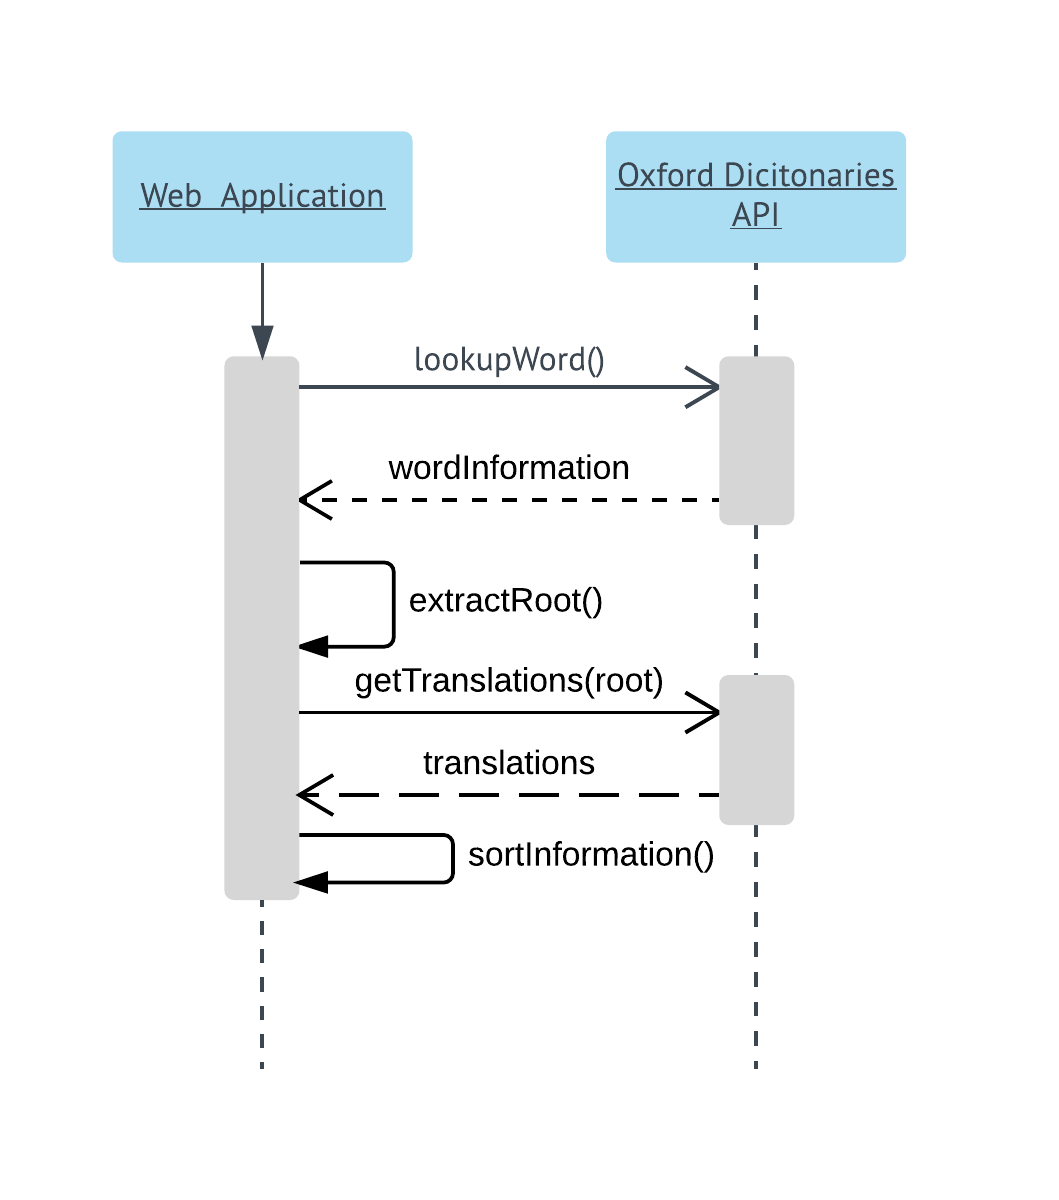
\includegraphics[width=0.7\textwidth]{Graphics/SystemsFlowOxford}
\end{center}
\end{figure}

On the first call, the root word, as provided by SpaCy, had it's translations looked up. If one or more translation was discovered, the second call would be made, extracting the grammatical information about why the root was transformed into it's current form. Both this grammatical information and the tag explanation from SpaCy were used in the final gloss.

Once this part of the application had been written, it was unit tested with a selection of random German words, the unconjugated word, translations and lexical information were compared to results provided by the other technologies and the developer's knowledge. The code passed testing as the results provided were accurate and contained the necessary grammatical information. 
	